\newpage
\section{Testes e Resultados}

\providecommand{\espacoreservado}[3]{\fbox{\parbox[c][#1][c]{#2}{\centering #3}}}

\par Este capítulo descreve a bancada montada para validar o sistema com equipamentos reais: os equipamentos, a comunicação, a configuração do inversor, o programa do controlador, o cadastro no supervisório, os ensaios e seus resultados.

\subsection{Objetivo e Visão Geral}

\par A bancada submete o sistema a um cenário realista, com um controlador lógico programável (\sigla{clp}), um inversor de frequência e um motor elétrico em funcionamento. O processo é simples: ligar, desligar e mudar a velocidade do motor, que fornece grandezas elétricas reais, como frequência, corrente e tensão.

\par O supervisório lê essas grandezas e o estado do motor, exibe-os em telas e gráficos, sinaliza alarmes e permite ligar e desligar o motor e alterar a referência de frequência. A Figura~\ref{fig:cap6_bancada_montada} reserva o espaço para a foto da bancada.

\begin{figure}[H]
    \centering
    \caption{Bancada de teste montada.}
    \label{fig:cap6_bancada_montada}
    \espacoreservado{6cm}{0.76\textwidth}{Espaço reservado para a fotografia da bancada completa (painel com o CLP, o inversor de frequência e o motor).}
    \vspace{0.2cm} \\
    Fonte: Autor.
\end{figure}

\todo[inline]{Inserir a fotografia da bancada montada em Imagens/Desenvolvimento/Cap5/ e trocar o espaço reservado por \texttt{\textbackslash includegraphics}. Informar o local (laboratório do instituto) e a data da montagem.}

\subsection{Equipamentos Utilizados}

\par A Tabela~\ref{tab:cap6_equipamentos} resume os itens da bancada.

{\renewcommand{\arraystretch}{1.3}\small
\begin{xltabular}{\textwidth}{>{\centering\arraybackslash}p{4.2cm}>{\centering\arraybackslash}X}
        \caption{Equipamentos da bancada de teste.}
        \label{tab:cap6_equipamentos}\\
        \hline
        \textbf{Equipamento} & \textbf{Função na bancada} \\
        \hline
        \endfirsthead
        \hline
        \textbf{Equipamento} & \textbf{Função na bancada} \\
        \hline
        \endhead
        \endfoot
        \multicolumn{2}{c}{Fonte: Autor.} \\
        \endlastfoot
        Servidor & Executa o supervisório \\
        \hline
        Rede local & Interliga o servidor e o \sigla{clp} \\
        \hline
        \sigla{clp} TM221 & Executa a lógica da bancada e responde ao supervisório por Modbus \\
        \hline
        Inversor ATV320 & Aciona o motor \\
        \hline
        Motor & Equipamento comandado na bancada \\
        \hline
\end{xltabular}}

\subsection{Arquitetura de Comunicação}

\par A comunicação tem dois segmentos independentes. No primeiro, a aquisição consulta o \sigla{clp} por Modbus, pela rede Ethernet \cite{MODBUS_TCP_IMPLEMENTATION_GUIDE}. No segundo, o \sigla{clp} consulta o inversor por Modbus, em um enlace serial \sigla{rs485} \cite{MODBUS_SERIAL_SPEC}. O \sigla{clp} é, portanto, servidor para o supervisório e mestre para o inversor, organização encontrada em instalações reais.

\par Na topologia da Figura~\ref{fig:cap6_topologia}, o servidor envia requisições Modbus ao \sigla{clp} pelo switch da rede local (1 e 2), e o \sigla{clp} responde com os valores em palavras e bits de memória. Em paralelo, o \sigla{clp} troca dados com o inversor por Modbus em \sigla{rs485} e comanda a partida e a parada por uma saída digital (3), e o inversor alimenta o motor (4).

\begin{figure}[H]
    \centering
    \caption{Topologia de comunicação da bancada.}
    \label{fig:cap6_topologia}
    \vspace{0.4cm}
    \figpadrao{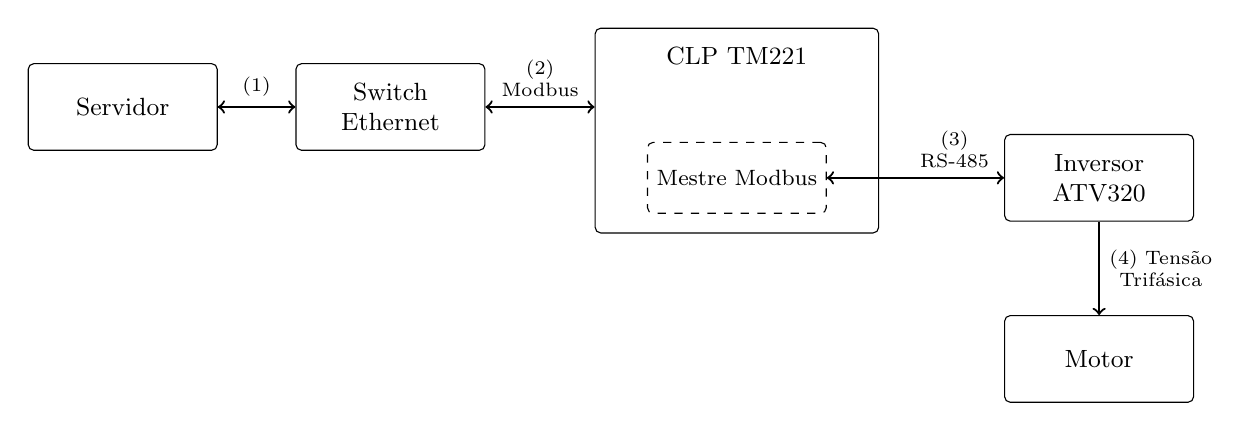
\begin{tikzpicture}[
        bloco/.style={draw, rectangle, rounded corners=2pt, minimum height=1.1cm, minimum width=2.4cm, align=center, font=\small},
        logico/.style={draw, dashed, rectangle, rounded corners=2pt, minimum height=0.9cm, minimum width=2.4cm, align=center, font=\footnotesize},
        enlace/.style={->, thick},
        rotulo/.style={font=\scriptsize, align=center}
    ]
        \node[bloco] (srv) at (0,0.3) {Servidor};
        \node[bloco] (sw) at (3.4,0.3) {Switch\\Ethernet};
        \node[bloco, minimum width=3.6cm, minimum height=2.6cm] (clp) at (7.8,0) {};
        \node[font=\small, align=center] at (7.8,0.95) {CLP TM221};
        \node[logico, minimum width=2cm] (mestre) at (7.8,-0.6) {Mestre Modbus};
        \node[bloco] (inv) at (12.4,-0.6) {Inversor\\ATV320};
        \node[bloco] (mot) at (12.4,-2.9) {Motor};

        \draw[enlace, <->] (srv) -- node[above, rotulo] {(1)} (sw);
        \draw[enlace, <->] (sw.east) -- node[above, rotulo] {(2)\\Modbus} (clp.west |- sw.east);
        \draw[enlace, <->] (mestre.east) -- node[above, rotulo, pos=0.72] {(3)\\RS-485} (inv.west);
        \draw[enlace] (inv) -- node[right, rotulo] {(4) Tensão\\Trifásica} (mot);
    \end{tikzpicture}}
    \vspace{0.2cm} \\
    Fonte: Autor.
\end{figure}

\par No segmento Ethernet, as palavras (\texttt{\%MW}) e os bits de memória (\texttt{\%M}) são acessíveis pelos mesmos endereços numéricos, contados a partir de zero: \texttt{\%MW0} é o registrador de retenção de endereço 0 e \texttt{\%M0} é a bobina de endereço 0 \cite{SCHNEIDER_MACHINE_EXPERT_BASIC}.

\par No segmento serial, o \sigla{clp} lê e escreve os registradores do inversor, como mostra a ligação da Figura~\ref{fig:cap6_foto_rs485}.

\begin{figure}[H]
    \centering
    \caption{Ligação serial RS-485 entre o CLP e o inversor.}
    \label{fig:cap6_foto_rs485}
    \espacoreservado{5cm}{0.76\textwidth}{Espaço reservado para a fotografia da ligação RS-485 entre o CLP e o inversor.}
    \vspace{0.2cm} \\
    Fonte: Autor.
\end{figure}

\subsection{Configuração do Inversor ATV320}

\par O inversor recebe o comando de partida e de parada por uma entrada digital e a referência de frequência pela comunicação Modbus. A Tabela~\ref{tab:cap6_params_atv320} lista os parâmetros.

{\renewcommand{\arraystretch}{1.3}\small
\begin{xltabular}{\textwidth}{>{\centering\arraybackslash}p{4.6cm}>{\centering\arraybackslash}p{3.6cm}>{\centering\arraybackslash}X}
        \caption{Parâmetros do ATV320.}
        \label{tab:cap6_params_atv320}\\
        \hline
        \textbf{Parâmetro} & \textbf{Valor} & \textbf{Finalidade} \\
        \hline
        \endfirsthead
        \hline
        \textbf{Parâmetro} & \textbf{Valor} & \textbf{Finalidade} \\
        \hline
        \endhead
        \endfoot
        \multicolumn{3}{c}{Fonte: Autor.} \\
        \endlastfoot
        Endereço Modbus & 2 & Identifica o inversor na rede serial \\
        \hline
        Taxa de transmissão Modbus & 19200 bit/s & Velocidade do enlace \sigla{rs485} \\
        \hline
        Formato Modbus & 8 bits, paridade par, 1 bit de parada (8E1) & Formato padrão do Modbus serial \cite{MODBUS_SERIAL_SPEC} \\
        \hline
        Tempo limite Modbus & 10 s & Falha de comunicação se o mestre deixar de consultar \\
        \hline
        Canal de comando 1 & Entrada digital & O comando de marcha e parada vem de uma saída digital do \sigla{clp} \\
        \hline
        Canal de referência 1 & Modbus & A referência de frequência vem da rede \\
        \hline
        Rampas de aceleração e de desaceleração & 5 s & Suaviza a partida e a parada do motor \\
        \hline
        Frequência mínima e máxima & 0 Hz e 50 Hz & Faixa de operação do motor \\
        \hline
\end{xltabular}}

\todo[inline]{Conferir os valores da Tabela~\ref{tab:cap6_params_atv320} no inversor.}

\par O \sigla{clp} lê do inversor a frequência, a corrente, a tensão, a potência e a rotação do motor e escreve a referência de frequência.

\par As Figuras~\ref{fig:cap6_foto_mebasic} e~\ref{fig:cap6_foto_atv320} mostram a configuração manual do controlador e do inversor.

\begin{figure}[H]
    \centering
    \caption{Configuração da comunicação serial no EcoStruxure Machine Expert Basic.}
    \label{fig:cap6_foto_mebasic}
    \espacoreservado{5.5cm}{0.76\textwidth}{Espaço reservado para a captura de tela do Machine Expert Basic (configuração da comunicação e do programa do CLP).}
    \vspace{0.2cm} \\
    Fonte: Autor.
\end{figure}

\begin{figure}[H]
    \centering
    \caption{Parametrização do inversor ATV320.}
    \label{fig:cap6_foto_atv320}
    \espacoreservado{5.5cm}{0.76\textwidth}{Espaço reservado para a fotografia do display do inversor ou captura do software de configuração mostrando os parâmetros de comunicação.}
    \vspace{0.2cm} \\
    Fonte: Autor.
\end{figure}

\subsection{Programa do Controlador}

\par O programa do \sigla{clp} executa, a cada ciclo, a comunicação com o inversor, a lógica de comando e a publicação dos resultados, como mostra a Figura~\ref{fig:cap6_blocos_clp}.

\begin{figure}[H]
    \centering
    \caption{Blocos funcionais do programa do CLP.}
    \label{fig:cap6_blocos_clp}
    \vspace{0.4cm}
    \figpadrao{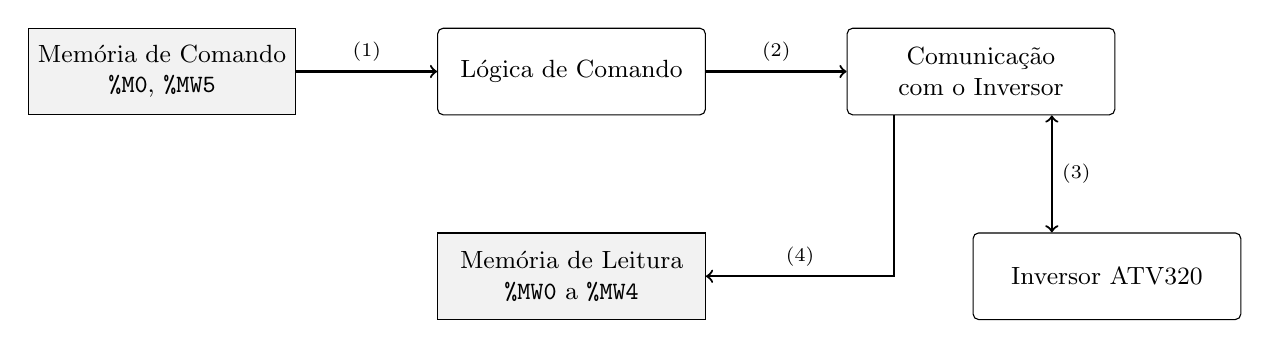
\begin{tikzpicture}[
        bloco/.style={draw, rectangle, rounded corners=2pt, minimum height=1.1cm, minimum width=3.4cm, align=center, font=\small},
        mem/.style={draw, rectangle, minimum height=1.1cm, minimum width=3.4cm, align=center, font=\small, fill=black!5},
        fluxo/.style={->, thick},
        rotulo/.style={font=\scriptsize, align=center}
    ]
        \node[mem] (cmd) at (0,2.6) {Memória de Comando\\\texttt{\%M0}, \texttt{\%MW5}};
        \node[bloco] (logica) at (5.2,2.6) {Lógica de Comando};
        \node[bloco] (com) at (10.4,2.6) {Comunicação\\com o Inversor};
        \node[mem] (pub) at (5.2,0) {Memória de Leitura\\\texttt{\%MW0} a \texttt{\%MW4}};
        \node[bloco] (inv) at (12.0,0) {Inversor ATV320};
        \coordinate (curva4) at ([xshift=-1.1cm]com.south |- pub.east);

        \draw[fluxo] (cmd) -- node[above, rotulo] {(1)} (logica);
        \draw[fluxo] (logica) -- node[above, rotulo] {(2)} (com);
        \draw[fluxo, <->] ([xshift=0.9cm]com.south) -- node[right, rotulo] {(3)} ([xshift=0.9cm]com.south |- inv.north);
        \draw[fluxo] ([xshift=-1.1cm]com.south) -- (curva4) -- node[above, rotulo] {(4)} (pub.east);
    \end{tikzpicture}}
    \vspace{0.2cm} \\
    Fonte: Autor.
\end{figure}

\par O supervisório escreve o comando e a referência na memória do controlador (1), e a lógica de comando aciona a saída digital do inversor e envia a referência ao bloco de comunicação (2). O bloco transfere a referência e traz a frequência, a corrente, a tensão, a potência e a rotação (3), publicadas nas posições de leitura (4).

\par A Tabela~\ref{tab:cap6_memoria_clp} reúne o mapa de memória, em que \texttt{\%M0} é a bobina de endereço 0 e \texttt{\%MW0} é o registrador de endereço 0. Os valores analógicos são inteiros, e o supervisório reconstrói o valor de engenharia por uma escala linear.

{\renewcommand{\arraystretch}{1.3}\small
\begin{xltabular}{\textwidth}{>{\centering\arraybackslash}p{3.4cm}>{\centering\arraybackslash}p{2.2cm}>{\centering\arraybackslash}X}
        \caption{Mapa de memória do CLP.}
        \label{tab:cap6_memoria_clp}\\
        \hline
        \textbf{Endereço} & \textbf{Tipo} & \textbf{Conteúdo} \\
        \hline
        \endfirsthead
        \hline
        \textbf{Endereço} & \textbf{Tipo} & \textbf{Conteúdo} \\
        \hline
        \endhead
        \endfoot
        \multicolumn{3}{c}{Fonte: Autor.} \\
        \endlastfoot
        \texttt{\%M0} & Bit & Comando liga/desliga escrito pelo supervisório, enviado ao inversor por uma saída digital \\
        \hline
        \texttt{\%MW0} & Palavra & Frequência de saída \\
        \hline
        \texttt{\%MW1} & Palavra & Corrente do motor \\
        \hline
        \texttt{\%MW2} & Palavra & Tensão de saída \\
        \hline
        \texttt{\%MW3} & Palavra & Potência \\
        \hline
        \texttt{\%MW4} & Palavra & Rotação (RPM) \\
        \hline
        \texttt{\%MW5} & Palavra & Referência de frequência escrita pelo supervisório \\
        \hline
\end{xltabular}}

\subsection{Configuração no Supervisório}

\par O cadastro no supervisório é feito pela interface, sem alteração de código.

\par A planta recebe o nome da bancada e as coordenadas do local. O dispositivo corresponde ao \sigla{clp}, com protocolo Modbus, endereço \sigla{ip} na rede local, porta 502 e o identificador de unidade do controlador, como resume a Tabela~\ref{tab:cap6_cadastro}.

{\renewcommand{\arraystretch}{1.3}\small
\begin{xltabular}{\textwidth}{>{\centering\arraybackslash}p{4.2cm}>{\centering\arraybackslash}X}
        \caption{Cadastro da bancada no sistema.}
        \label{tab:cap6_cadastro}\\
        \hline
        \textbf{Item} & \textbf{Valor} \\
        \hline
        \endfirsthead
        \hline
        \textbf{Item} & \textbf{Valor} \\
        \hline
        \endhead
        \endfoot
        \multicolumn{2}{c}{Fonte: Autor.} \\
        \endlastfoot
        Planta & Bancada do motor \\
        \hline
        Coordenadas da planta & Latitude $-$26,8815 e longitude $-$49,1365 (Instituto Federal Catarinense, Campus Blumenau) \\
        \hline
        Dispositivo de E/S & \sigla{clp} TM221, protocolo Modbus \\
        \hline
        Endereço \sigla{ip} e porta & Endereço do \sigla{clp} na rede local, porta 502 \\
        \hline
        Identificador de unidade & 1 \\
        \hline
        Tempo limite e tentativas & Padrões do sistema (1000 ms e 2 tentativas) \\
        \hline
\end{xltabular}}

\par Cada tag traz o mapeamento Modbus, o tipo bruto e a escala, e o período de varredura é o do dispositivo, de 1 s. Como os valores são inteiros em décimos, a escala linear leva, por exemplo, o intervalo bruto de 0 a 500 ao de 0 a 50 hertz, na frequência. A Tabela~\ref{tab:cap6_tags} apresenta as sete tags.

{\renewcommand{\arraystretch}{1.3}\small
\begin{xltabular}{\textwidth}{>{\centering\arraybackslash}p{2.6cm}>{\centering\arraybackslash}p{2.8cm}>{\centering\arraybackslash}p{2.3cm}>{\centering\arraybackslash}p{1.7cm}>{\centering\arraybackslash}X}
        \caption{Tags cadastradas no sistema para a bancada.}
        \label{tab:cap6_tags}\\
        \hline
        \textbf{Nome} & \textbf{Endereço Modbus} & \textbf{Tipo bruto} & \textbf{Unidade} & \textbf{Formato} \\
        \hline
        \endfirsthead
        \hline
        \textbf{Nome} & \textbf{Endereço Modbus} & \textbf{Tipo bruto} & \textbf{Unidade} & \textbf{Formato} \\
        \hline
        \endhead
        \endfoot
        \multicolumn{5}{c}{Fonte: Autor.} \\
        \endlastfoot
        Frequência de saída & Registrador de retenção 0 (\texttt{\%MW0}) & Inteiro 16 bits sem sinal & Hz & Analógico \\
        \hline
        Corrente do motor & Registrador de retenção 1 (\texttt{\%MW1}) & Inteiro 16 bits sem sinal & A & Analógico \\
        \hline
        Tensão de saída & Registrador de retenção 2 (\texttt{\%MW2}) & Inteiro 16 bits sem sinal & V & Analógico \\
        \hline
        Potência & Registrador de retenção 3 (\texttt{\%MW3}) & Inteiro 16 bits sem sinal & kW & Analógico \\
        \hline
        Rotação & Registrador de retenção 4 (\texttt{\%MW4}) & Inteiro 16 bits sem sinal & RPM & Analógico \\
        \hline
        Comando liga/desliga & Bobina 0 (\texttt{\%M0}) & Digital, leitura e escrita & n/a & Simples \\
        \hline
        Referência de frequência & Registrador de retenção 5 (\texttt{\%MW5}) & Inteiro 16 bits sem sinal, leitura e escrita & Hz & Analógico \\
        \hline
\end{xltabular}}

\par As tags de comando liga/desliga e de referência aceitam escrita, sempre pelo diálogo de comando. Como o comando é bem-sucedido com a resposta do controlador, sem releitura, a confirmação do efeito real vem da leitura posterior da frequência.

\par Um alarme de corrente alta é configurado sobre a corrente do motor, com limite [A CONFIRMAR] e banda morta, para evitar disparos repetidos, e o evento de falha de comunicação do dispositivo pode ser ligado a um alarme comum.

\todo[inline]{Confirmar com o autor se o alarme da bancada é o de corrente alta, com o limite, a severidade e a banda morta conforme o motor. Registrar o nome exato dos eventos e dos alarmes criados.}

\par O sinótico representa o motor por um símbolo de onde se abre o diálogo de comando, com a frequência, a corrente, a tensão, a potência e a rotação em indicadores. O \emph{dashboard} reúne um gráfico da frequência e da corrente e um medidor, e a lista de acompanhamento mostra as sete tags. A Figura~\ref{fig:cap6_telas_movi} reserva o espaço para essas telas.

\begin{figure}[H]
    \centering
    \caption{Telas de supervisão da bancada.}
    \label{fig:cap6_telas_movi}
    \espacoreservado{6cm}{0.76\textwidth}{Espaço reservado para as capturas do sinótico do motor e do \emph{dashboard} com o gráfico de frequência e corrente.}
    \vspace{0.2cm} \\
    Fonte: Autor.
\end{figure}

\todo[inline]{Montar o sinótico, o dashboard e a lista de acompanhamento no sistema e inserir as capturas em Imagens/Desenvolvimento/Cap5/. Descrever o desenho do sinótico efetivamente criado (objetos, vínculos de animação e cores).}

\subsection{Ensaios e Resultados}

\par Seis ensaios exercitam, em sequência, a leitura contínua com o motor desligado, a partida e a parada pelo supervisório, o alarme de corrente alta e seu reconhecimento, a perda e o retorno de comunicação e a troca da referência de frequência. Eles estão na Tabela~\ref{tab:cap6_ensaios}. Duas medidas interessam: o tempo entre a confirmação do comando e a resposta do equipamento, que mede a latência do caminho de escrita, e o atraso do supervisório, entre uma mudança no equipamento e sua exibição na tela, limitado pela soma do período de varredura, do período de atualização da tela e de uma margem de processamento (RNF01).

{\renewcommand{\arraystretch}{1.3}\small
\begin{xltabular}{\textwidth}{cXX}
        \caption{Ensaios da bancada.}
        \label{tab:cap6_ensaios}\\
        \hline
        \textbf{Id} & \textbf{Ensaio} & \textbf{Requisitos verificados} \\
        \hline
        \endfirsthead
        \hline
        \textbf{Id} & \textbf{Ensaio} & \textbf{Requisitos verificados} \\
        \hline
        \endhead
        \endfoot
        \multicolumn{3}{c}{Fonte: Autor.} \\
        \endlastfoot
        E1 & Leitura contínua com o motor desligado & RF01, RF02, RF03, RF04, RNF01 \\
        \hline
        E2 & Partida pelo supervisório & RF06, RF08, RNF01 \\
        \hline
        E3 & Parada pelo supervisório & RF06, RF08, RF17, RNF01 \\
        \hline
        E4 & Alarme de corrente alta e reconhecimento & RF16, RF17, RNF05 \\
        \hline
        E5 & Perda de comunicação e retorno & RF01, RF03, RF16 \\
        \hline
        E6 & Troca da referência de frequência & RF06, RF08, RNF05 \\
        \hline
\end{xltabular}}

\par \emph{Ensaio E1.} Com o motor parado, as grandezas não variam, o que isola o desempenho da aquisição. O ensaio mantém as tags em leitura contínua e confere se o histórico não perde amostras, se o carimbo de tempo é monotônico e espaçado pelo período configurado, com variação de poucos milissegundos, e se a lista de acompanhamento atrasa no máximo o período de varredura mais o de atualização da tela. Espera-se uma taxa de entrega próxima de 100\,\% e nenhum alarme.

\par \emph{Ensaio E2.} O operador define a referência de 40 hertz e envia o comando de partida. O sistema escreve a ordem em uma bobina do \sigla{clp}, que aciona o inversor por uma saída digital. O ensaio mede o tempo entre a confirmação e a resposta do \sigla{clp}, em que o comando é dado como concluído, e o tempo até a frequência começar a subir na tela. Espera-se a resposta em dezenas de milissegundos, bem abaixo do limite de 30 s do comando, que a trava por tag impeça um segundo comando simultâneo e que o comando fique registrado com o operador, a tag, o valor e o instante.

\par \emph{Ensaio E3.} A ordem de parada segue o mesmo caminho, e a frequência desce pela rampa de desaceleração. Espera-se o mesmo tempo de comando do E2, que a tela acompanhe a frequência até zero e que a leitura continue sem perda, sem alarme de comunicação, o que separa o efeito do processo do efeito do sistema.

\par \emph{Ensaio E4.} Com o motor ligado, a corrente cruza o limite configurado [A CONFIRMAR] do alarme de corrente alta, e o detector cria uma ocorrência. O ensaio mede o tempo entre o cruzamento e a exibição no indicador de alarmes, que deve ser da ordem do atraso do supervisório. O operador reconhece o alarme, e confere-se que o registro guarda o nome e o instante. Parado o motor, a corrente cai abaixo do limite, descontada a banda morta, e o alarme retorna ao normal. Espera-se um alarme único por cruzamento e a sequência correta na linha do tempo.

\par \emph{Ensaio E5.} A comunicação é interrompida desconectando o cabo Ethernet entre o comutador e o \sigla{clp}, e depois restabelecida. Durante a falha, o \sigla{clp} continua executando o programa. O sistema marca o valor como desatualizado depois de três períodos de varredura, mantendo o último valor e o carimbo, e o dispositivo passa a degradado depois de três ciclos falhos. Com o cabo de volta, o primeiro ciclo bem-sucedido fecha o estado, sem rajada de leituras acumuladas. O ensaio mede o tempo até a marcação de desatualizado e o tempo até a volta à qualidade boa e confere que não há lacuna preenchida no histórico, pois a lacuna é a evidência da falha.

\par \emph{Ensaio E6.} Com o motor a 40 hertz, o operador altera a referência para 30 hertz pelo mesmo comando. O ensaio mede o tempo até a resposta do \sigla{clp} e até a frequência atingir a referência, e confere que um segundo comando imediato é recusado pela trava por tag e que o reenvio do mesmo pedido não cria uma segunda escrita.

\par A Tabela~\ref{tab:cap6_medidas} reúne as medidas previstas.

{\renewcommand{\arraystretch}{1.3}\small
\begin{xltabular}{\textwidth}{cXcc}
        \caption{Medidas previstas nos ensaios da bancada.}
        \label{tab:cap6_medidas}\\
        \hline
        \textbf{Ensaio} & \textbf{Medida} & \textbf{Esperado} & \textbf{Medido} \\
        \hline
        \endfirsthead
        \hline
        \textbf{Ensaio} & \textbf{Medida} & \textbf{Esperado} & \textbf{Medido} \\
        \hline
        \endhead
        \endfoot
        \multicolumn{4}{c}{Fonte: Autor.} \\
        \endlastfoot
        E1 & Taxa de leituras gravadas em relação às esperadas & acima de 99\,\% & a medir \\
        \hline
        E1 & Variação do intervalo entre carimbos consecutivos & poucos ms & a medir \\
        \hline
        E1 & Atraso do supervisório (equipamento até a tela) & varredura mais atualização da tela & a medir \\
        \hline
        E2 & Confirmação do operador até a resposta do CLP à escrita & dezenas de ms & a medir \\
        \hline
        E2 & Resposta do CLP até a primeira mudança de frequência na tela & varredura mais atualização da tela & a medir \\
        \hline
        E2 & Duração da rampa de aceleração observada & valor configurado no inversor & a medir \\
        \hline
        E3 & Confirmação do operador até a resposta do CLP à escrita & dezenas de ms & a medir \\
        \hline
        E3 & Resposta do CLP até a frequência zero na tela & rampa de desaceleração mais atraso do supervisório & a medir \\
        \hline
        E3 & Leituras perdidas durante a transição & nenhuma & a medir \\
        \hline
        E4 & Cruzamento do limite até o alarme na tela & varredura mais atualização da tela & a medir \\
        \hline
        E4 & Ocorrências geradas por cruzamento & uma & a medir \\
        \hline
        E4 & Reconhecimento até o registro com nome e instante & imediato (próxima atualização da tela) & a medir \\
        \hline
        E5 & Interrupção até a marcação de desatualizado & três períodos de varredura & a medir \\
        \hline
        E5 & Interrupção até o estado de comunicação degradado & três ciclos falhos & a medir \\
        \hline
        E5 & Retorno do cabo até a qualidade boa na tela & um ciclo mais atualização da tela & a medir \\
        \hline
        E5 & Linhas gravadas no histórico durante a falha & nenhuma & a medir \\
        \hline
        E6 & Confirmação do operador até a resposta do CLP à escrita & dezenas de ms & a medir \\
        \hline
        E6 & Resposta do CLP até a frequência medida igual à referência & rampa do inversor mais atraso do supervisório & a medir \\
        \hline
        E6 & Segundo comando imediato na mesma tag & recusado pela trava & a medir \\
        \hline
        E6 & Reenvio do mesmo pedido & uma única escrita & a medir \\
        \hline
\end{xltabular}}

\todo[inline]{Conferir os parâmetros citados (referência de 40 e 30 Hz, rampas do inversor, limite de corrente) e medir e inserir, para cada ensaio, o gráfico da tela e os valores da Tabela~\ref{tab:cap6_medidas}. Informar as rampas do inversor, o registrador da referência, o período de varredura, a corrente em cada regime e a linha do registro de comandos. Confirmar a referência de 40 e 30 Hz e se o alarme de falha de comunicação foi ligado.}
